\documentclass[../main.tex]{subfiles}
\begin{document}


\appendix
\renewcommand{\chaptermark}[1]{\markboth{Appendix \thechapter\relax:\thinspace\relax#1}{}}
\chapter{Additional results}
\label{sec:additionalResults}


\section{Latent space similarity analysis}
\label{sec:add_lat}

\begin{figure}[ht!]
     \centering
    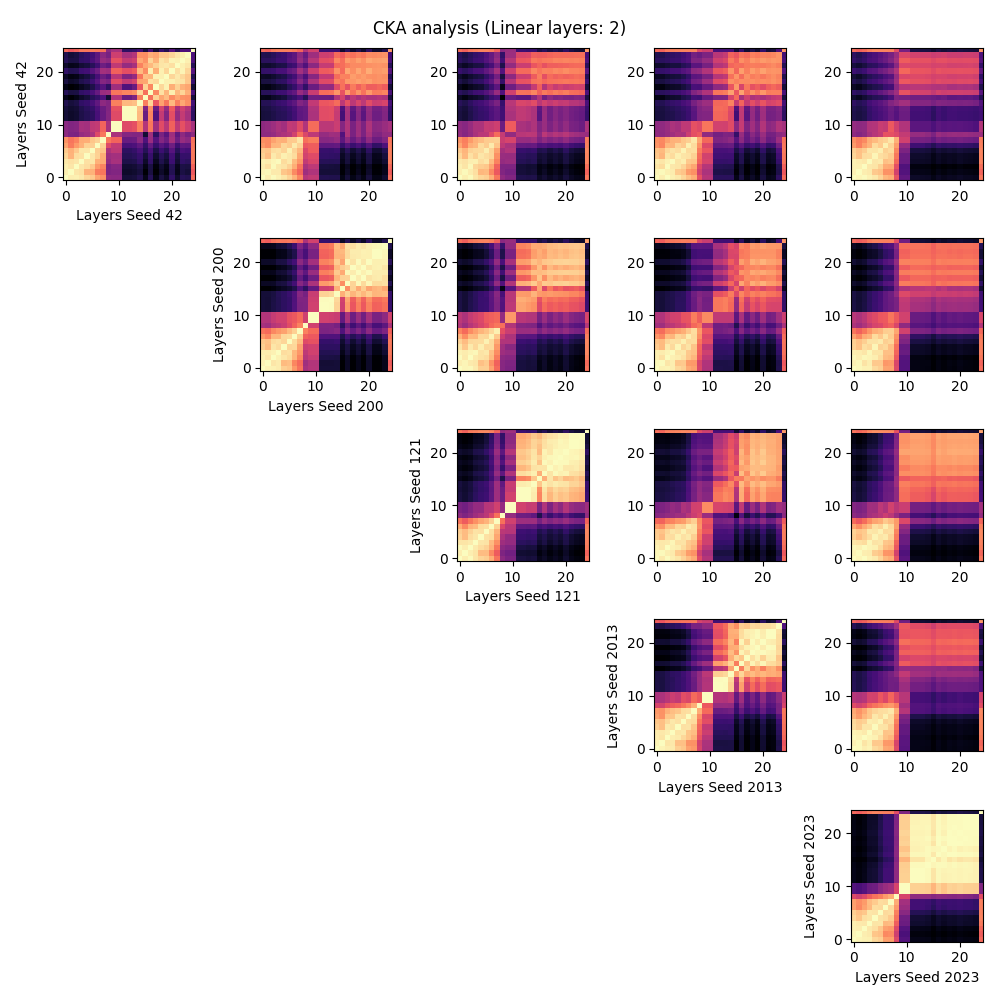
\includegraphics[width=0.84\textwidth]{figures/rs/sim_ae/cka_2__42_200_121_2013_2023.png} 
    \caption{Additional CKA analysis for the autoencoder with linear layers: 2}
    \label{fig:extra_cka_ae_2} 
\end{figure}
%
\begin{figure}[ht!]
    \centering
    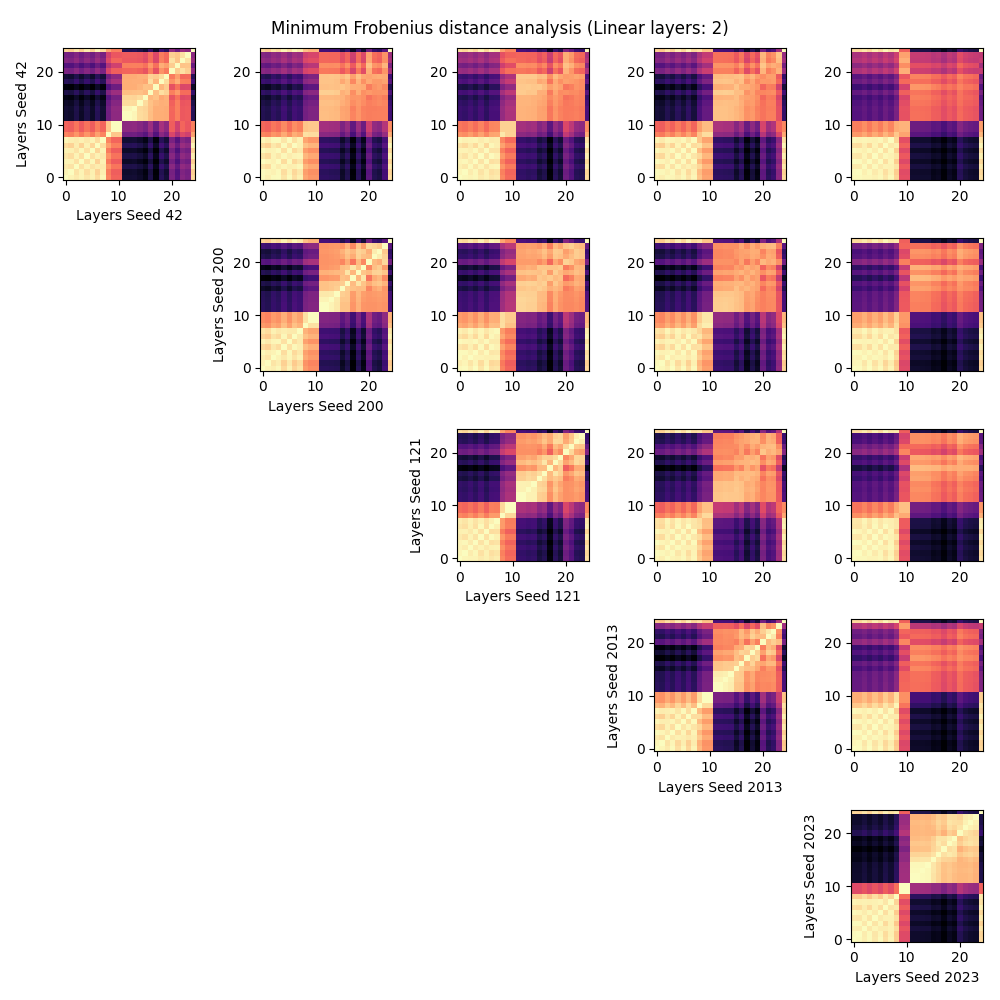
\includegraphics[width=\textwidth]{figures/rs/sim_ae/frob_2__42_200_121_2013_2023.png}
    \caption{Additional Min. Frobenius norm analysis for the autoencoder with linear layers: 2}
    \label{fig:extra_frob_ae_2}
\end{figure}
%
\begin{figure}[ht!]
    \centering
    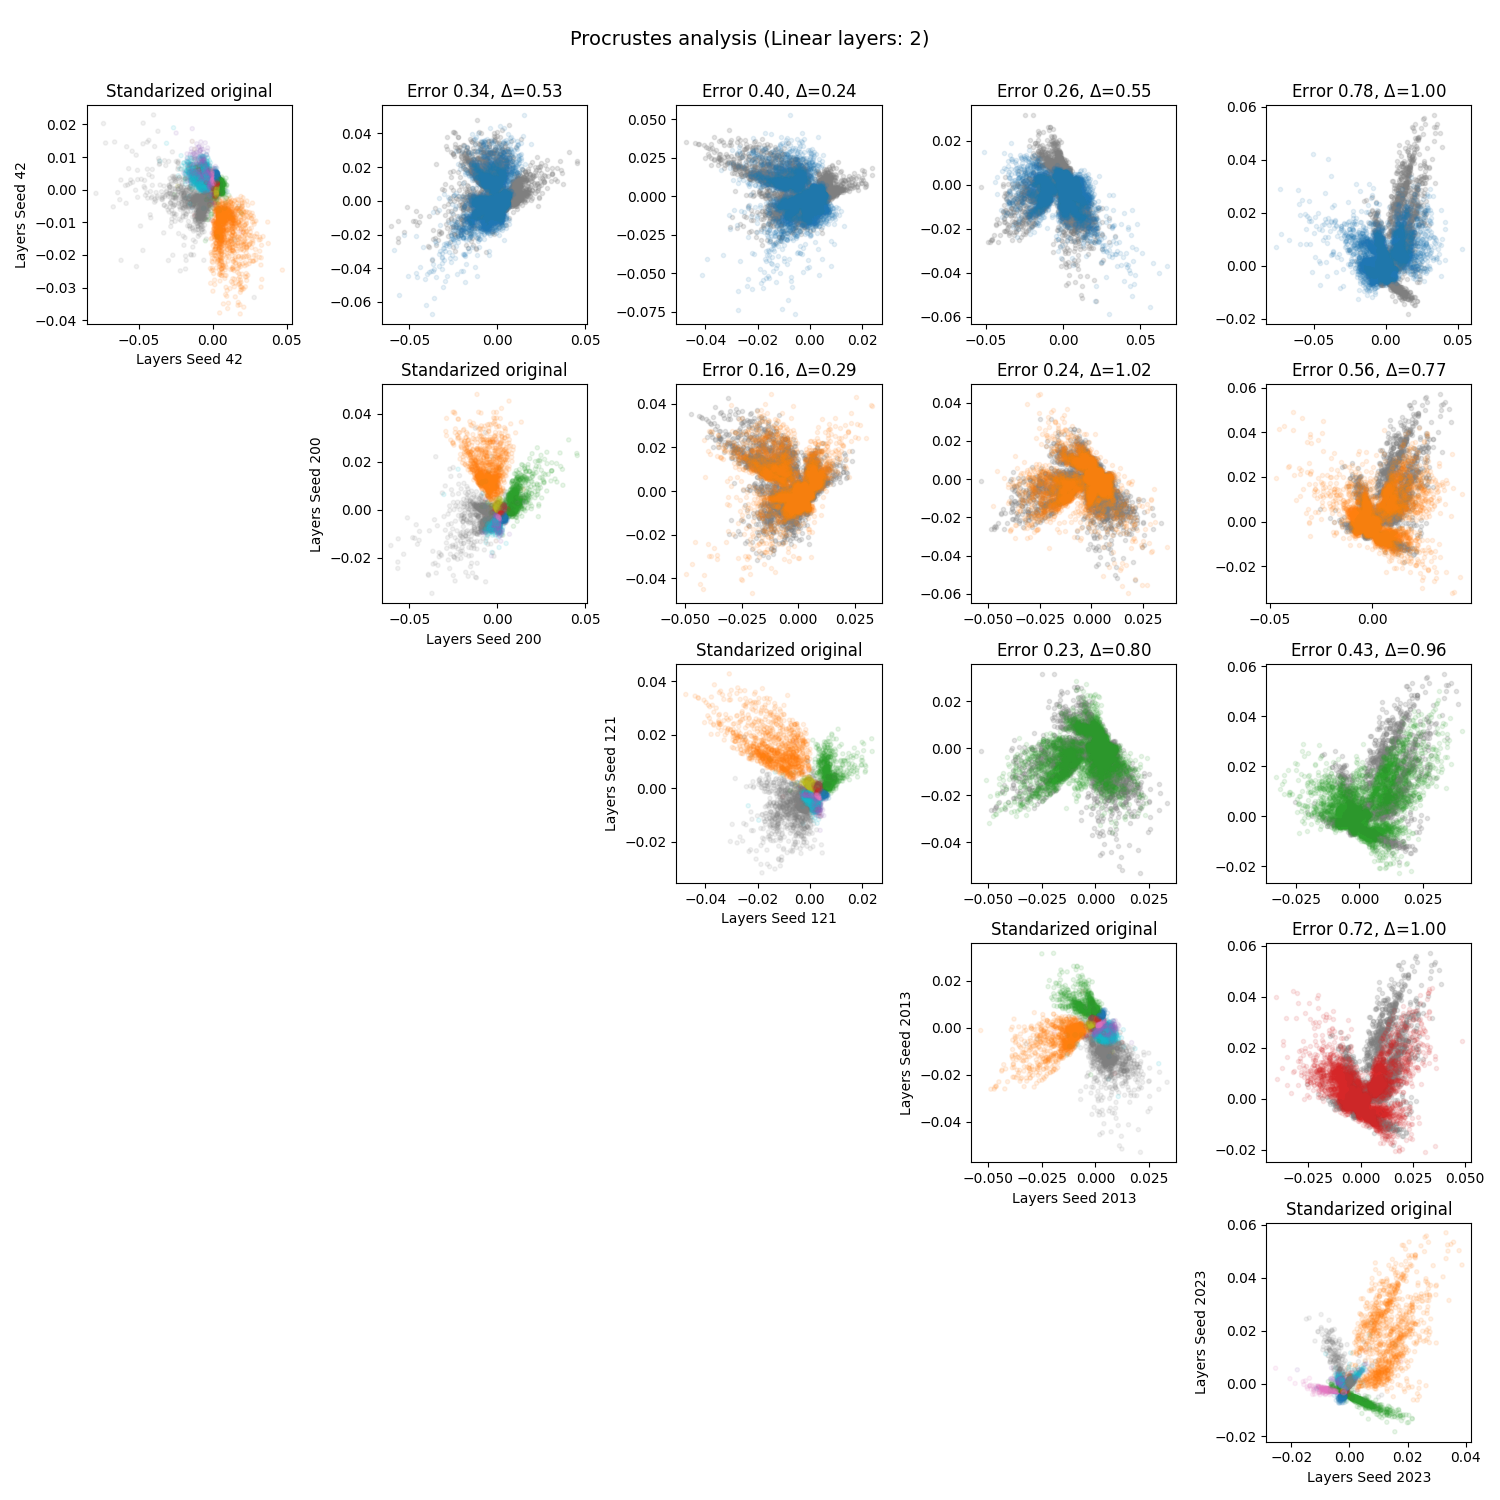
\includegraphics[width=\textwidth]{figures/rs/sim_ae/procrustes_2__42_200_121_2013_2023.png} 
    \caption{Additional Procrustes analysis for the autoencoder with linear layers: 2}
    \label{fig:extra_proc_ae_2}
\end{figure}
%
\begin{figure}[ht!]
     \centering
    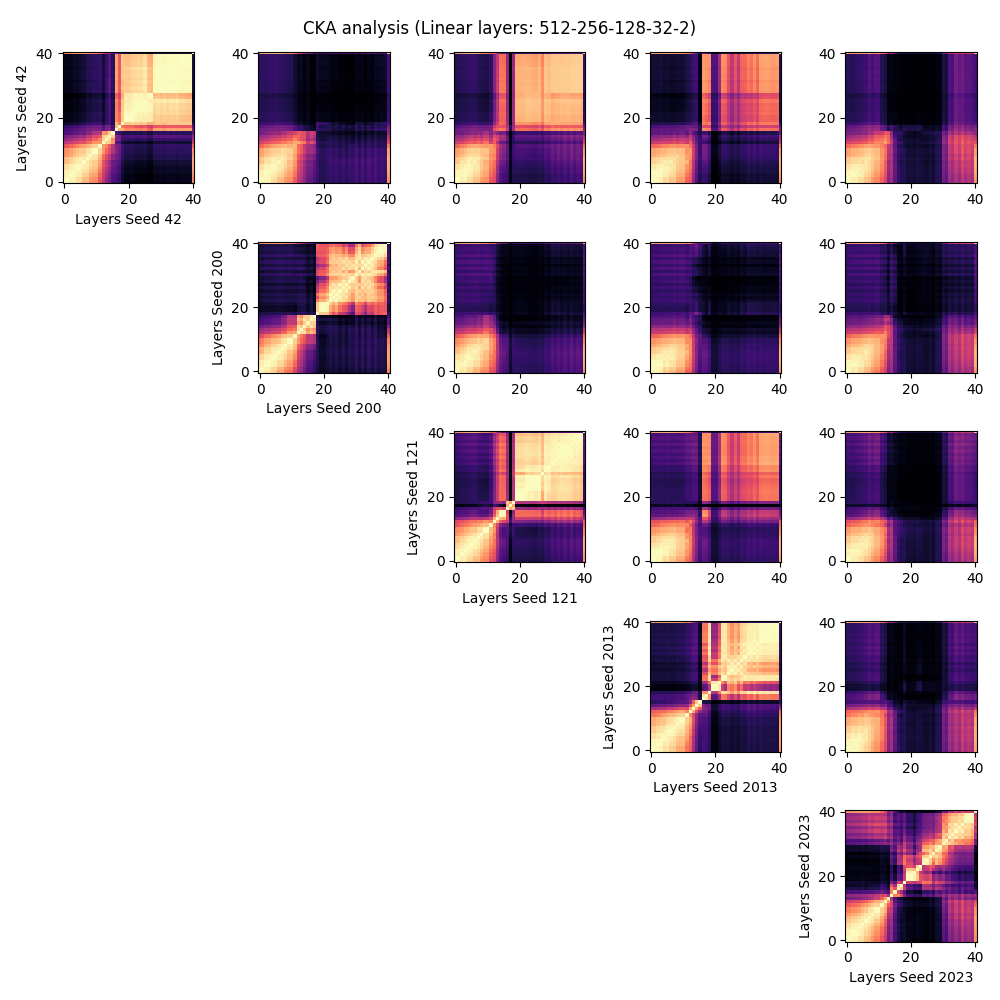
\includegraphics[width=\textwidth]{figures/rs/sim_ae/cka_512-256-128-32-2__42_200_121_2013_2023.png} 
    \caption{Additional CKA analysis for the autoencoder with linear layers: 512-256-128-32-2}
    \label{fig:extra_cka_ae_512_256_128_32_2}
\end{figure}
%
\begin{figure}[ht!]
    \centering
    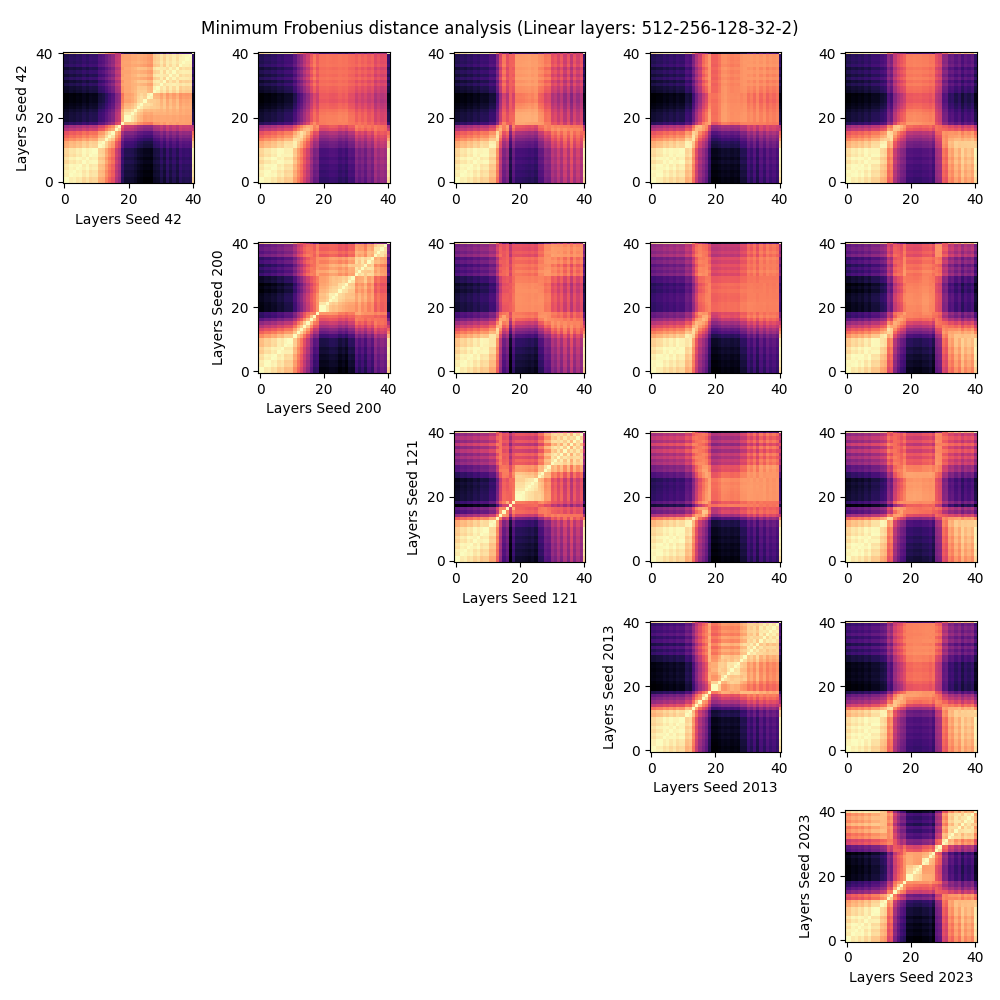
\includegraphics[width=\textwidth]{figures/rs/sim_ae/frob_512-256-128-32-2__42_200_121_2013_2023.png}
    \caption{Additional Min. Frobenius norm analysis for the autoencoder with linear layers: 512-256-128-32-2}
    \label{fig:extra_frob_ae_512_256_128_32_2}
\end{figure}
%
\begin{figure}[ht!]
    \centering
    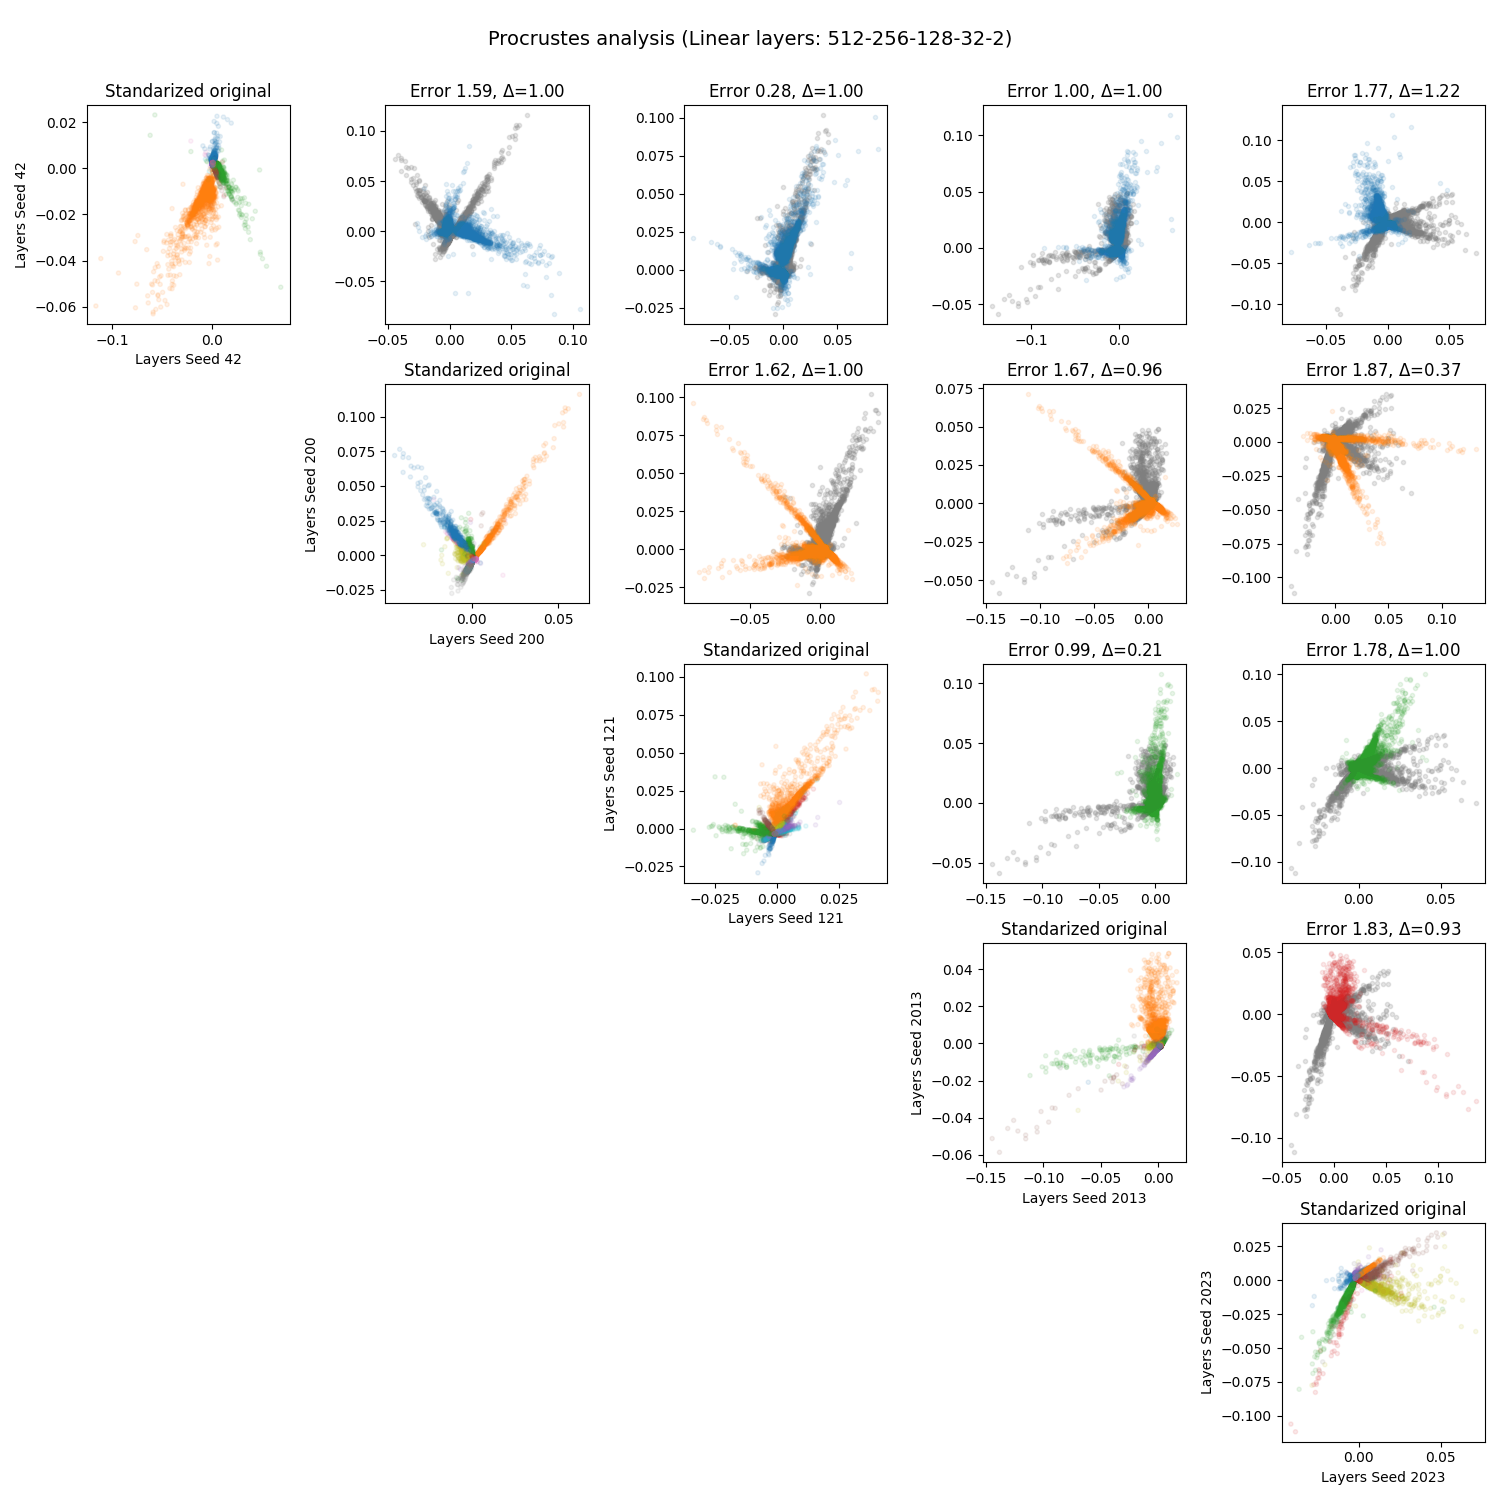
\includegraphics[width=\textwidth]{figures/rs/sim_ae/procrustes_512-256-128-32-2__42_200_121_2013_2023.png} 
    \caption{Additional Procrustes analysis for the autoencoder with linear layers: 512-256-128-32-2}
    \label{fig:extra_proc_ae_512_256_128_32_2}
\end{figure}
%
\begin{figure}[ht!]
     \centering
    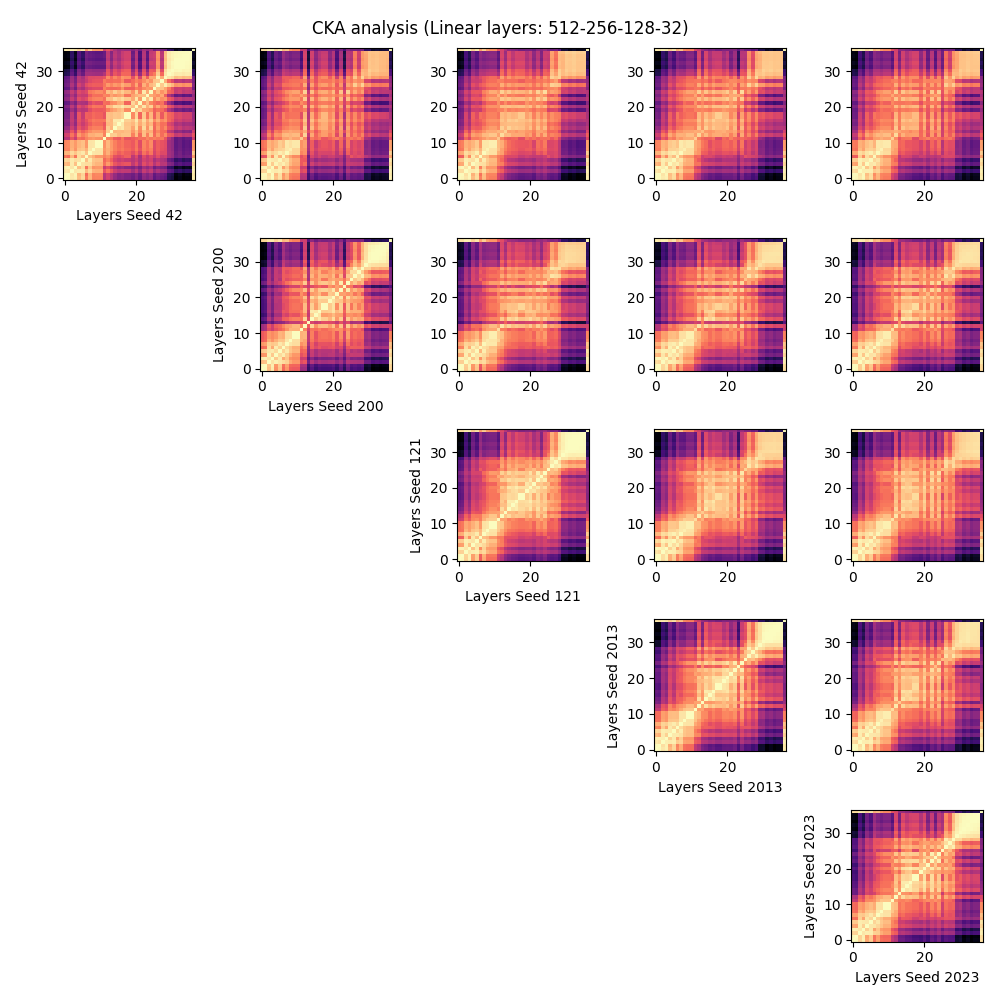
\includegraphics[width=\textwidth]{figures/rs/sim_ae/cka_512-256-128-32__42_200_121_2013_2023.png} 
    \caption{Additional CKA analysis for the autoencoder with linear layers: 512-256-128-32}
    \label{fig:extra_cka_ae_512_256_128_32}
\end{figure}
%
\begin{figure}[ht!]
    \centering
    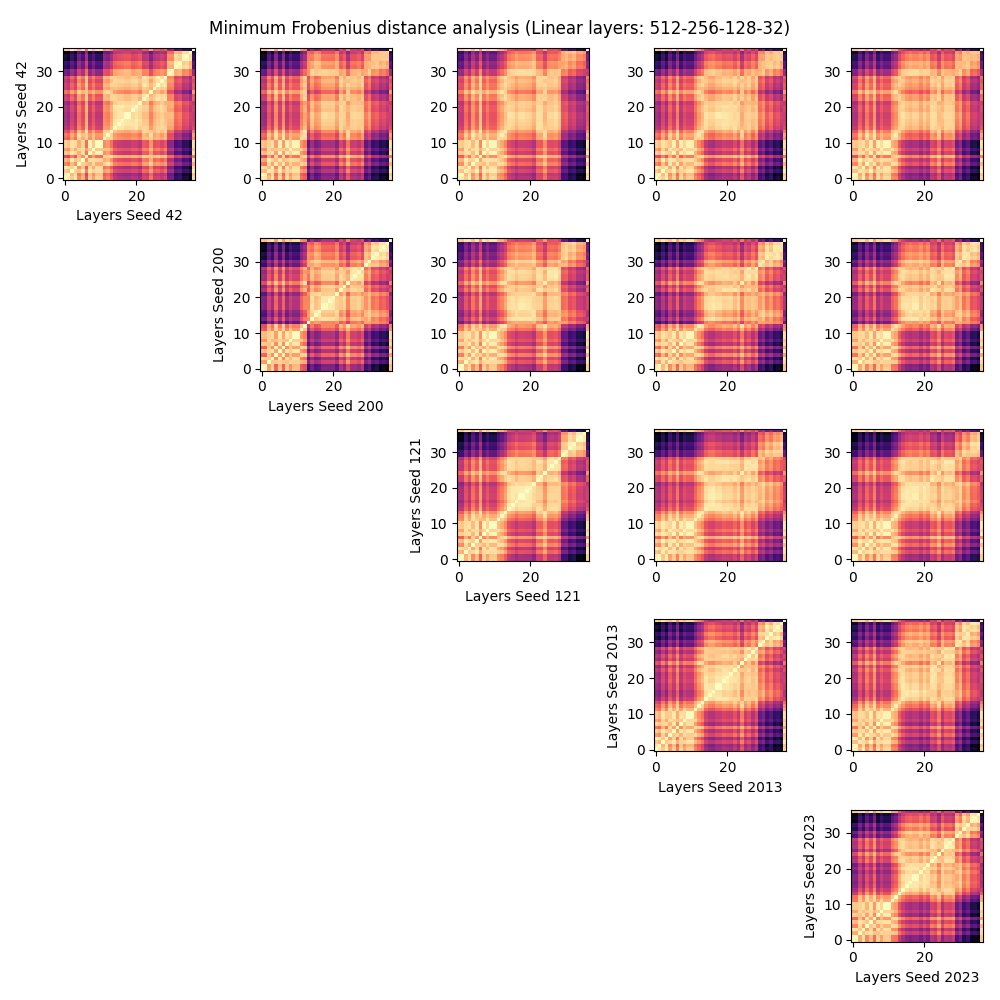
\includegraphics[width=0.9\textwidth]{figures/rs/sim_ae/frob_512-256-128-32__42_200_121_2013_2023.png}
    \caption{Additional Min. Frobenius norm analysis for the autoencoder with linear layers: 512-256-128-32}
    \label{fig:extra_frob_ae_512_256_128_32}
\end{figure}
%
\begin{figure}[ht!]
    \centering
    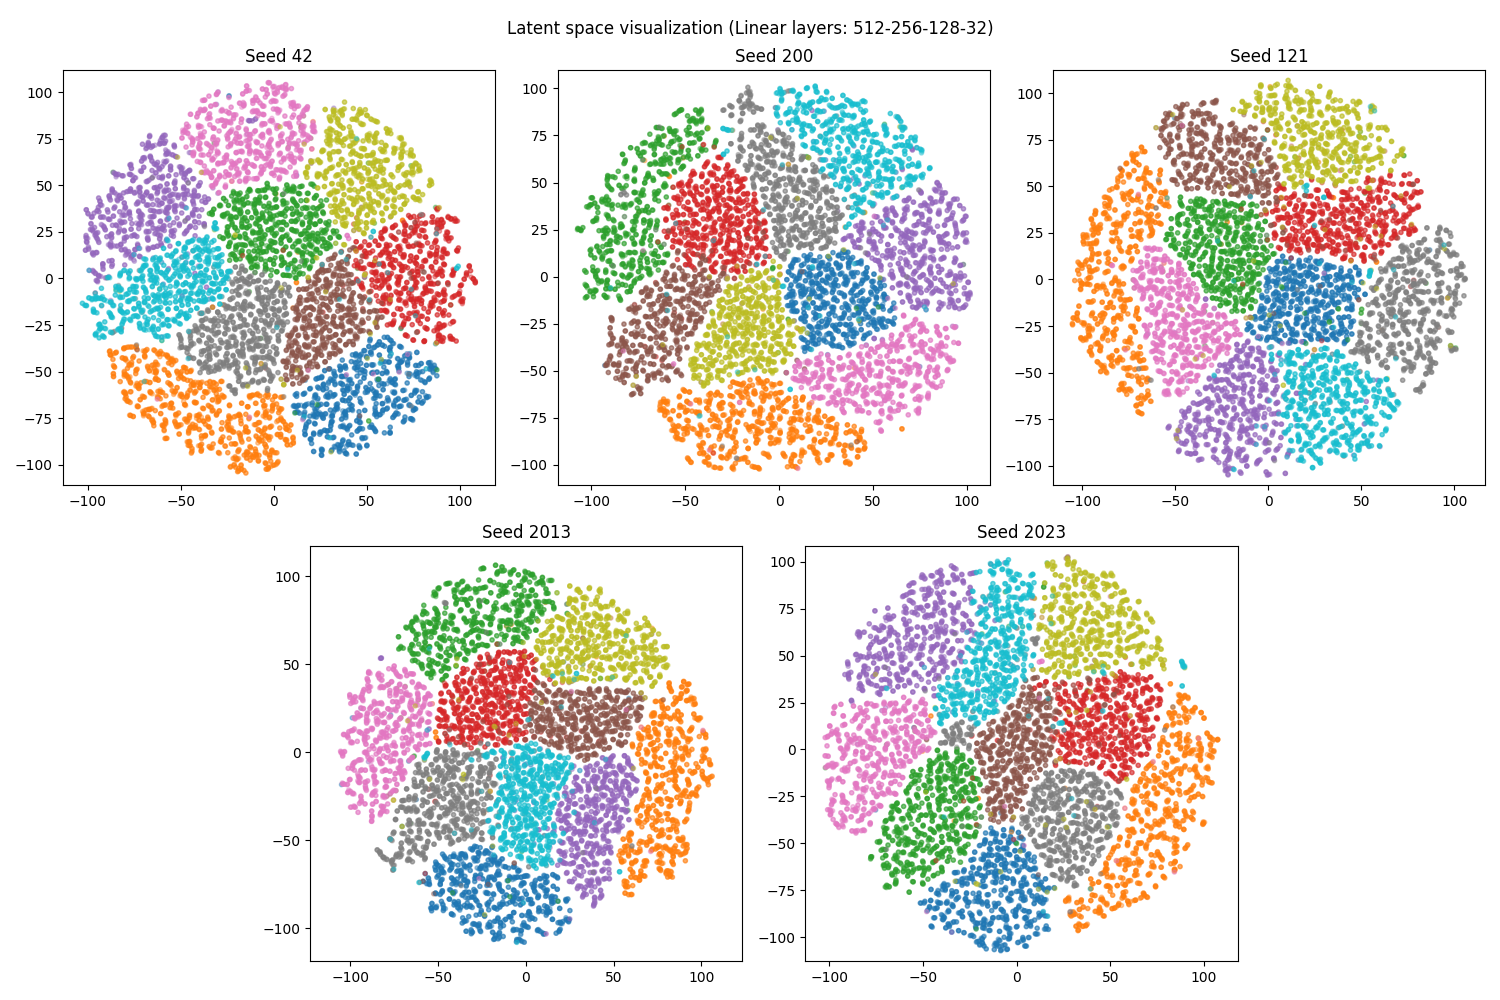
\includegraphics[width=0.7\textwidth]{figures/rs/sim_ae/vis_tsne_512-256-128-32__42_200_121_2013_2023.png} 
    \caption{T-SNE of the encoded latent space for the autoencoder with linear layers: 512-256-128-32}
    \label{fig:tsne_ae_512_256_128_32}
\end{figure}
%
\begin{figure}[ht!]
    \centering
    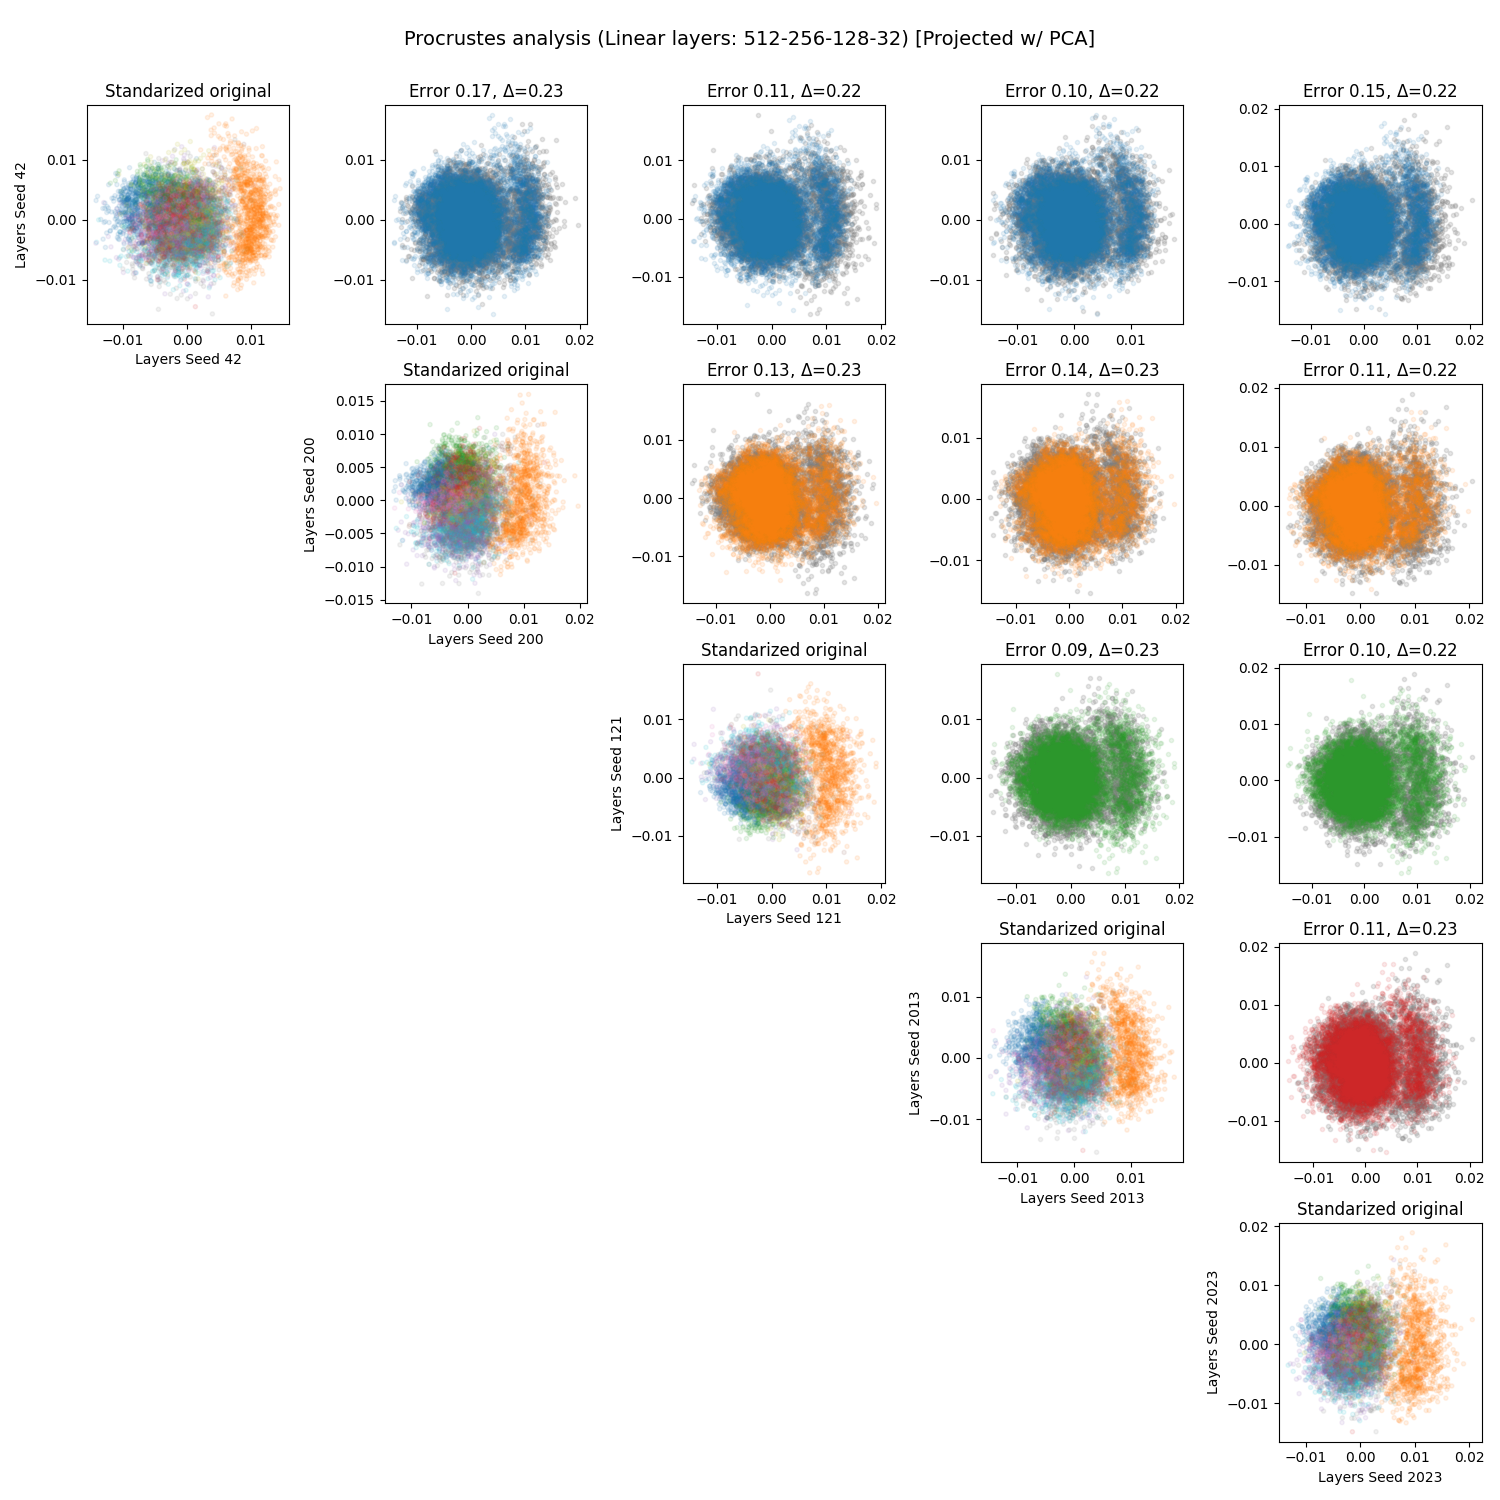
\includegraphics[width=\textwidth]{figures/rs/sim_ae/procrustes_512-256-128-32__42_200_121_2013_2023.png} 
    \caption{Additional Procrustes analysis for the autoencoder with linear layers: 512-256-128-32}
    \label{fig:extra_proc_ae_512_256_128_32}
\end{figure}
%
\begin{figure}[ht!]
     \centering
    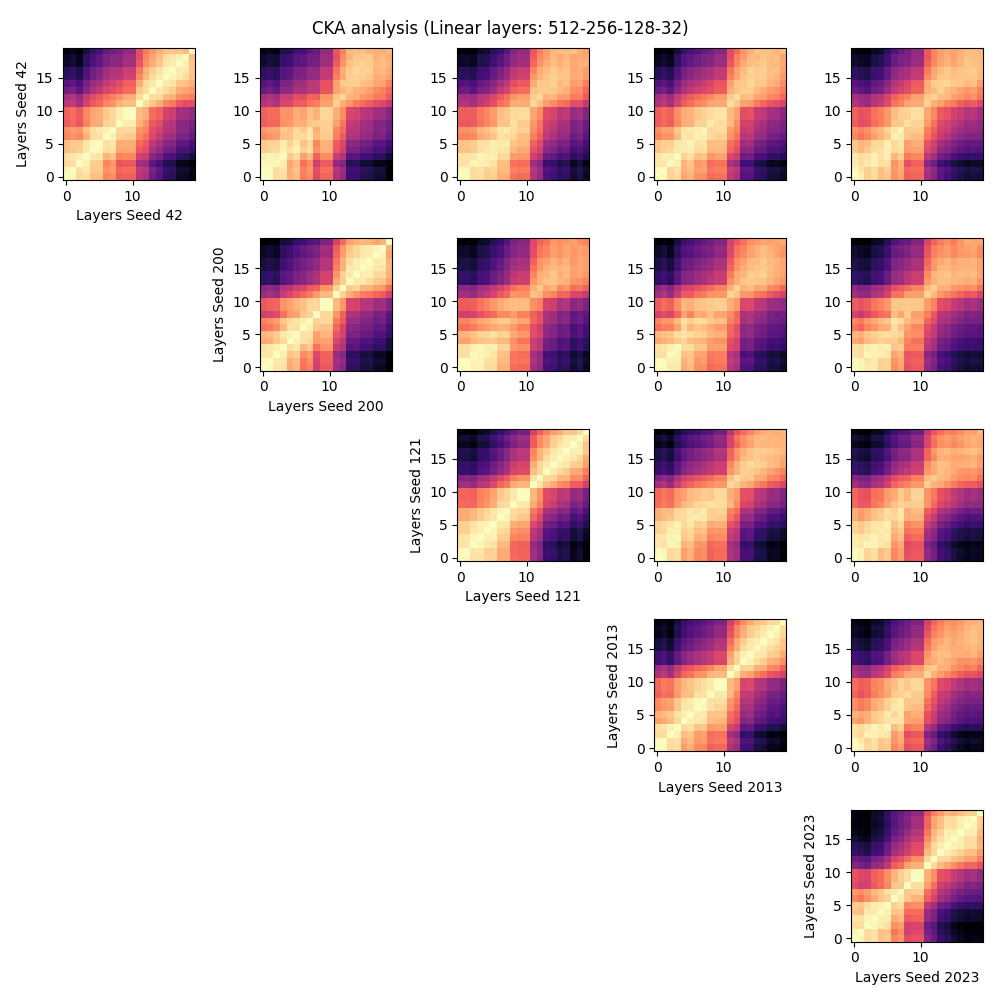
\includegraphics[width=\textwidth]{figures/rs/sim_cls/cka_512-256-128-32__42_200_121_2013_2023.png} 
    \caption{Additional CKA analysis for the CNN classifier}
    \label{fig:extra_cka_cls}
\end{figure}
%
\begin{figure}[ht!]
    \centering
    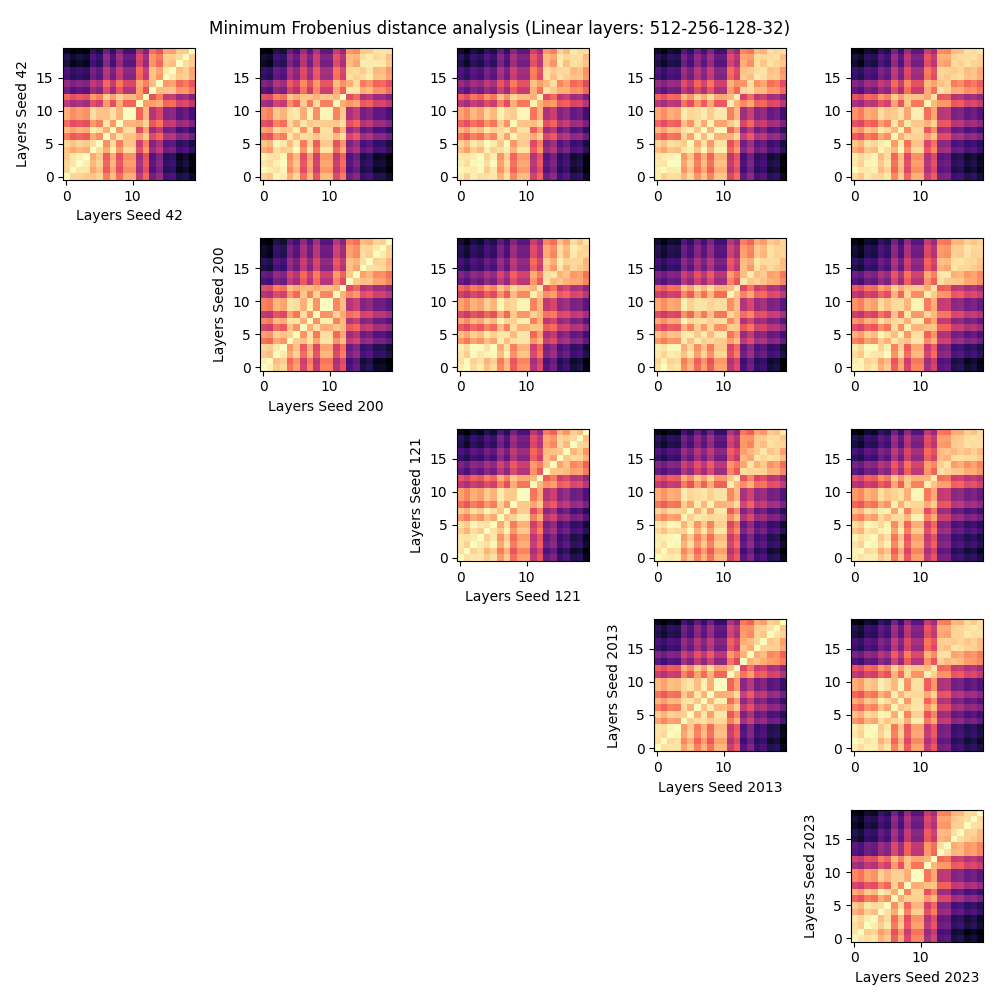
\includegraphics[width=0.9\textwidth]{figures/rs/sim_cls/frob_512-256-128-32__42_200_121_2013_2023.png}
    \caption{Additional Min. Frobenius norm analysis for the CNN classifier}
    \label{fig:extra_frob_cls}
\end{figure}
%
\begin{figure}[ht!]
    \centering
    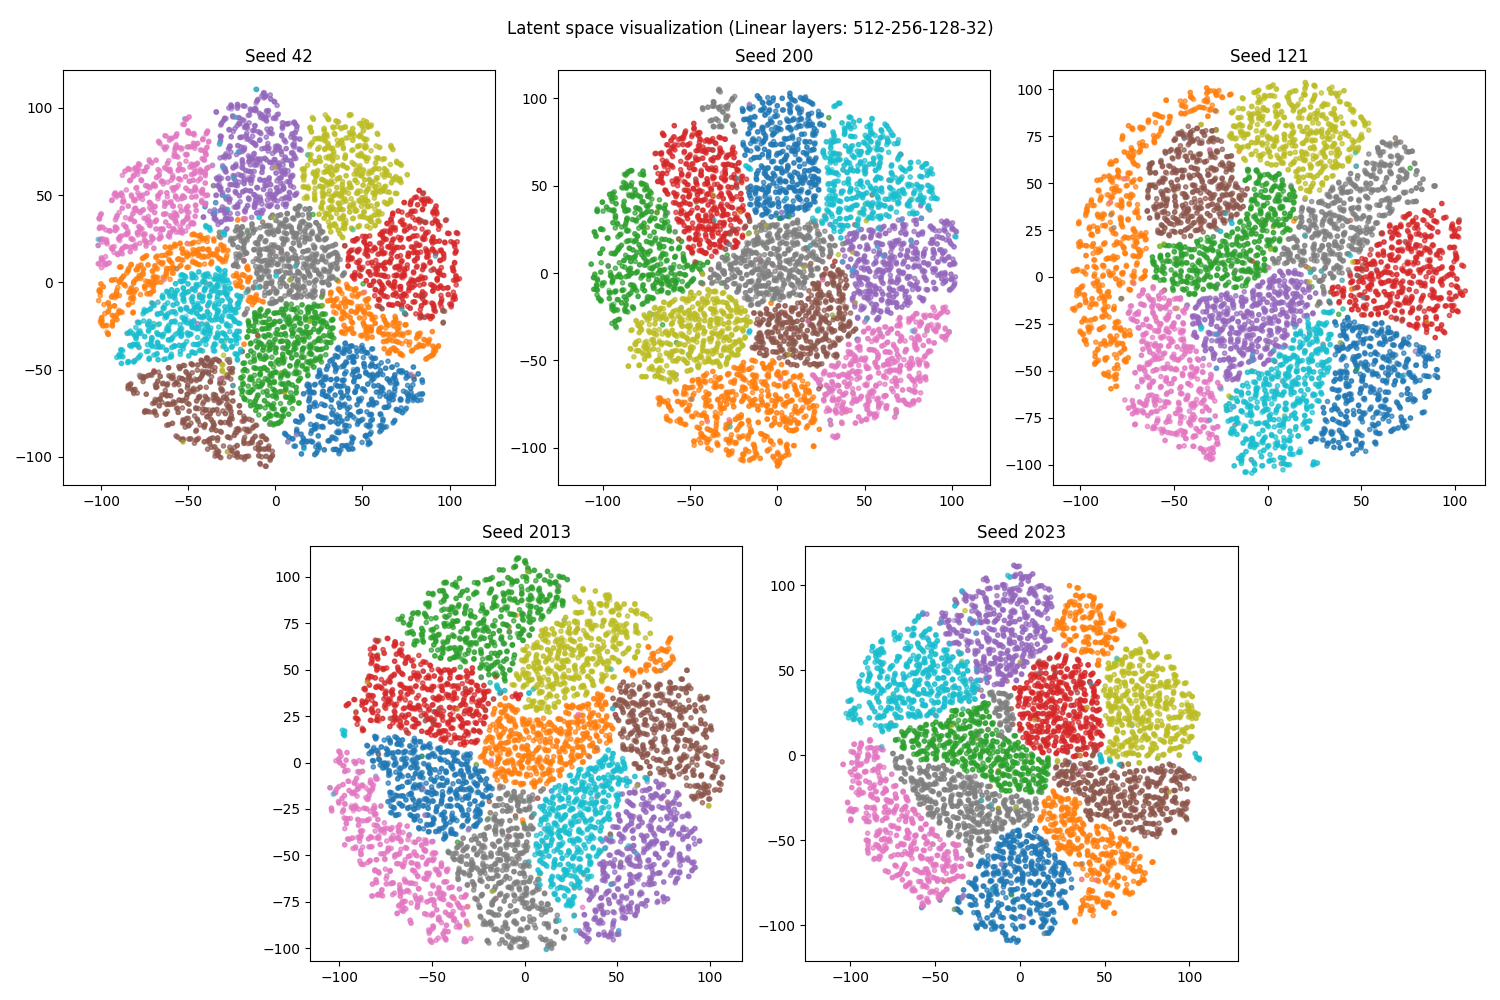
\includegraphics[width=0.7\textwidth]{figures/rs/sim_cls/vis_tsne_512-256-128-32__42_200_121_2013_2023.png} 
    \caption{T-SNE of the encoded latent space  for the CNN classifier}
    \label{fig:tsne_cls}
\end{figure}
%
\begin{figure}[ht!]
    \centering
    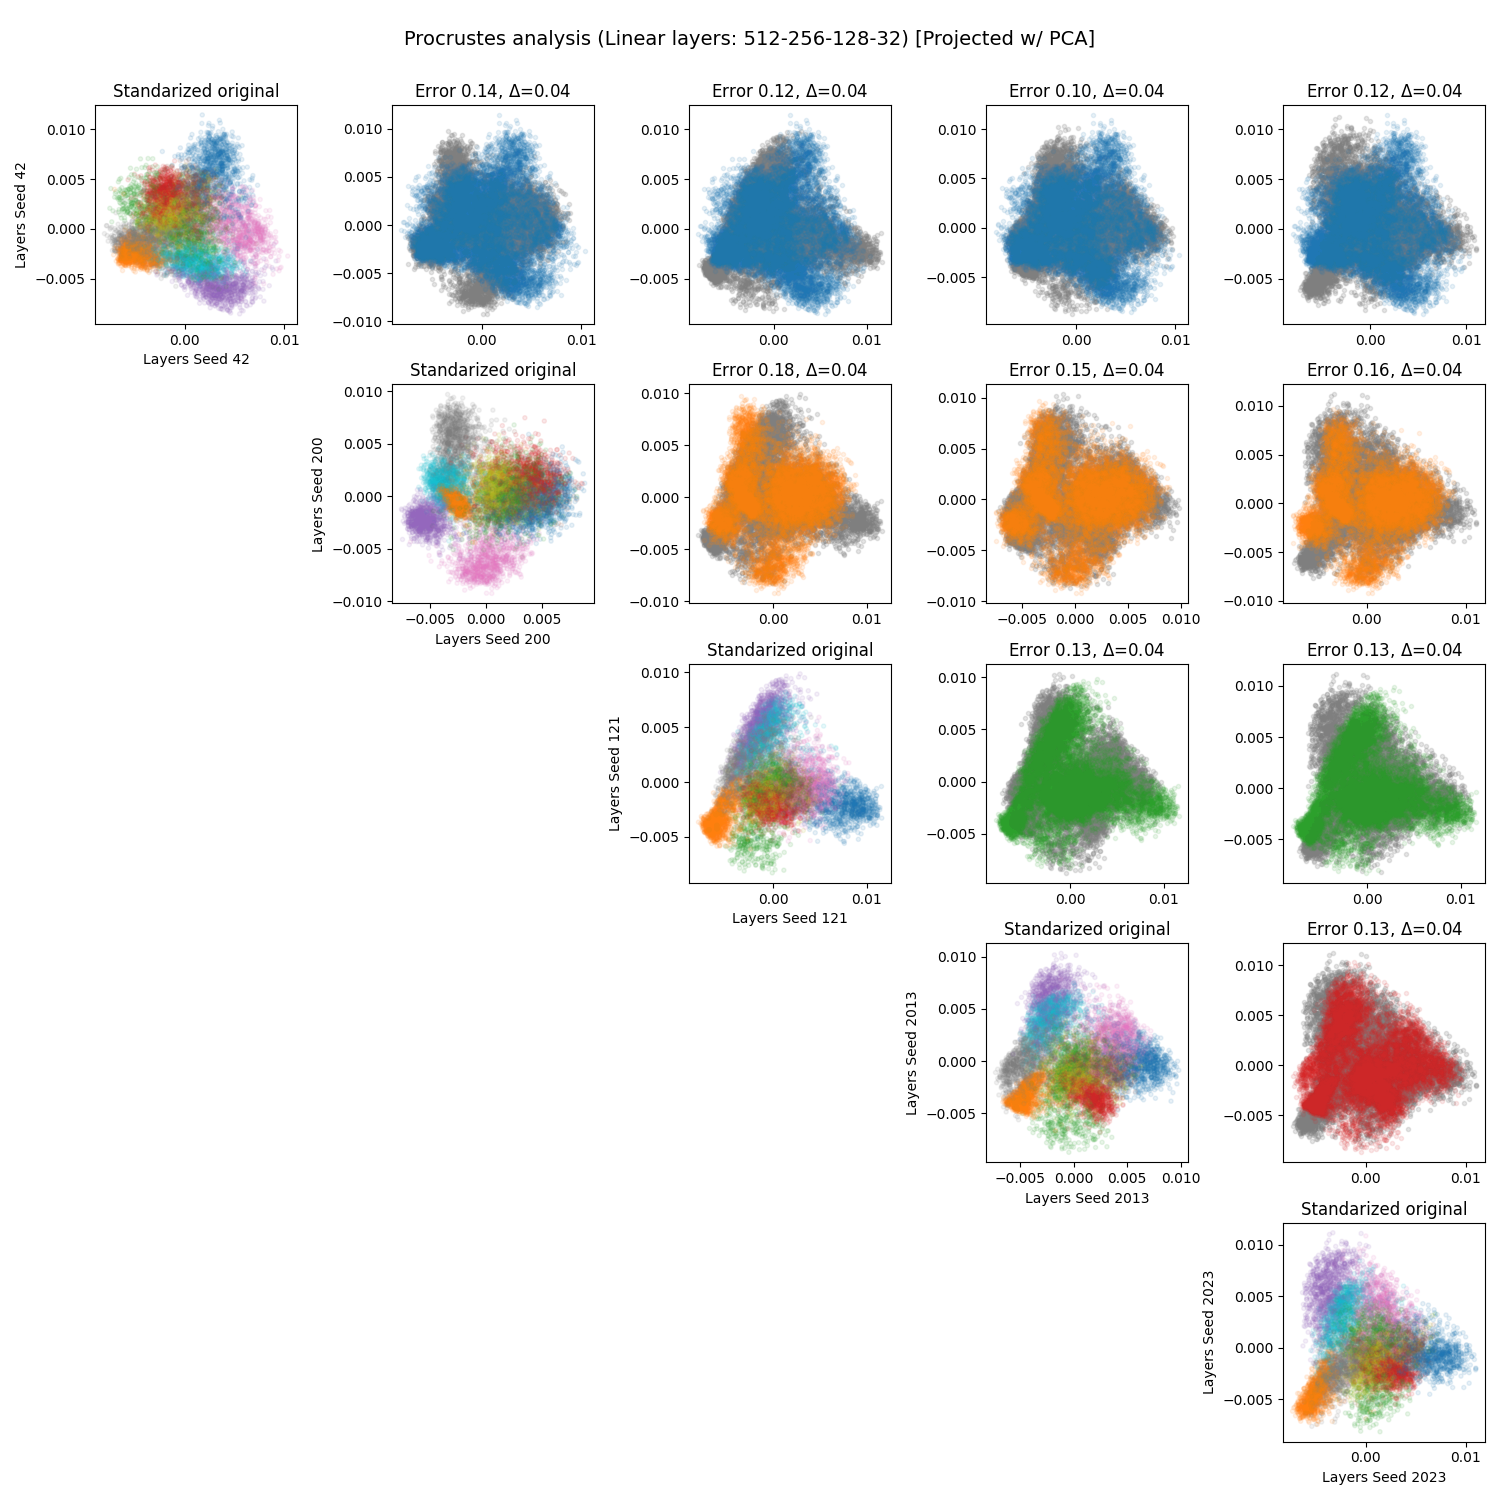
\includegraphics[width=\textwidth]{figures/rs/sim_cls/procrustes_512-256-128-32__42_200_121_2013_2023.png} 
    \caption{Additional Procrustes analysis for the CNN classifier}
    \label{fig:extra_proc_cls}
\end{figure}
%
\FloatBarrier
%
\section{Multilingual model stitching}

\begin{table}[ht!]
\centering
\resizebox{\textwidth}{!}{
\begin{tabular}{clcccccc}
\toprule
   &    & \multicolumn{3}{c}{Absolute} & \multicolumn{3}{c}{Relative} \\
 \cmidrule(lr){3-5} 
 \cmidrule(lr){6-8} 
 Decoder & Encoder & $\text{Acc} \times 100$ & $\text{FScore} \times 100$ & $\text{MAE} \times 100$ & $\text{Acc} \times 100$ & $\text{FScore} \times 100$ & $\text{MAE} \times 100$ \\
\midrule
\multirow{3}{*}{en} & en &  $92.00 \pm 0.07$ &  $92.00 \pm 0.07$ &   $8.00 \pm 0.07$ &  $89.24 \pm 1.79$ &  $89.24 \pm 1.79$ &  $10.76 \pm 1.79$ \\
   & es &  $49.91 \pm 0.02$ &  $33.32 \pm 0.02$ &  $50.09 \pm 0.02$ &  $83.70 \pm 1.48$ &  $83.66 \pm 1.52$ &  $16.30 \pm 1.48$ \\
   & fr &  $52.95 \pm 0.14$ &  $42.81 \pm 0.83$ &  $47.05 \pm 0.14$ &  $78.85 \pm 0.49$ &  $78.81 \pm 0.54$ &  $21.15 \pm 0.49$ \\
&\\
\multirow{3}{*}{es} & en &  $41.15 \pm 5.76$ &  $31.48 \pm 1.03$ &  $58.85 \pm 5.76$ &  $76.21 \pm 3.02$ &  $76.10 \pm 3.01$ &  $23.79 \pm 3.02$ \\
   & es &  $91.74 \pm 0.94$ &  $91.72 \pm 0.95$ &   $8.26 \pm 0.94$ &  $90.36 \pm 0.02$ &  $90.35 \pm 0.02$ &   $9.64 \pm 0.02$ \\
   & fr &  $47.81 \pm 1.15$ &  $43.70 \pm 2.93$ &  $52.19 \pm 1.15$ &  $77.26 \pm 0.90$ &  $77.22 \pm 0.92$ &  $22.74 \pm 0.90$ \\
&\\
\multirow{3}{*}{fr} & en &  $50.28 \pm 0.28$ &  $35.07 \pm 2.22$ &  $49.73 \pm 0.28$ &  $81.80 \pm 1.66$ &  $81.79 \pm 1.66$ &  $18.20 \pm 1.66$ \\
   & es &  $50.34 \pm 0.05$ &  $34.59 \pm 0.47$ &  $49.66 \pm 0.05$ &  $81.01 \pm 0.94$ &  $80.85 \pm 0.95$ &  $18.99 \pm 0.94$ \\
   & fr &  $87.62 \pm 0.85$ &  $87.60 \pm 0.89$ &  $12.38 \pm 0.85$ &  $85.61 \pm 0.62$ &  $85.60 \pm 0.62$ &  $14.39 \pm 0.62$ \\
\bottomrule
\end{tabular}
}
\caption{Coarse grained: finetune (over two random seeds)}
\label{tab:multilingual-finetune-coarse-grained}
\end{table}

\begin{table}[ht!]
\centering
\resizebox{\textwidth}{!}{
\begin{tabular}{clcccccc}
\toprule
   &    & \multicolumn{3}{c}{Absolute} & \multicolumn{3}{c}{Relative} \\
 \cmidrule(lr){3-5} 
 \cmidrule(lr){6-8} 
 Decoder & Encoder & $\text{Acc} \times 100$ & $\text{FScore} \times 100$ & $\text{MAE} \times 100$ & $\text{Acc} \times 100$ & $\text{FScore} \times 100$ & $\text{MAE} \times 100$ \\
\midrule
\multirow{3}{*}{en} & en &   $93.33 \pm 1.80$ &   $93.33 \pm 1.80$ &    $6.67 \pm 1.80$ &   $91.56 \pm 2.81$ &   $91.56 \pm 2.80$ &    $8.43 \pm 2.81$ \\
   & es &   $54.41 \pm 6.15$ &  $44.39 \pm 15.17$ &   $45.59 \pm 6.15$ &   $88.21 \pm 5.76$ &   $88.19 \pm 5.78$ &   $11.79 \pm 5.76$ \\
   & fr &  $41.82 \pm 15.29$ &  $34.55 \pm 11.59$ &  $58.18 \pm 15.29$ &   $85.00 \pm 8.59$ &   $84.97 \pm 8.62$ &   $15.00 \pm 8.59$ \\
&\\
\multirow{3}{*}{es} & en &   $45.30 \pm 8.25$ &   $37.10 \pm 8.05$ &   $54.69 \pm 8.25$ &  $83.22 \pm 10.71$ &  $83.15 \pm 10.77$ &  $16.78 \pm 10.71$ \\
   & es &   $93.20 \pm 1.79$ &   $93.20 \pm 1.80$ &    $6.79 \pm 1.79$ &   $92.01 \pm 2.25$ &   $92.00 \pm 2.25$ &    $7.99 \pm 2.25$ \\
   & fr &   $41.22 \pm 9.42$ &   $37.15 \pm 8.19$ &   $58.78 \pm 9.42$ &   $83.88 \pm 9.37$ &   $83.85 \pm 9.39$ &   $16.12 \pm 9.37$ \\
&\\
\multirow{3}{*}{fr} & en &   $50.20 \pm 0.26$ &   $34.69 \pm 1.79$ &   $49.80 \pm 0.26$ &   $87.02 \pm 6.69$ &   $87.01 \pm 6.69$ &   $12.98 \pm 6.69$ \\
   & es &   $52.56 \pm 3.07$ &   $40.35 \pm 8.05$ &   $47.44 \pm 3.07$ &   $86.18 \pm 7.40$ &   $86.08 \pm 7.49$ &   $13.82 \pm 7.40$ \\
   & fr &   $90.42 \pm 3.58$ &   $90.40 \pm 3.59$ &    $9.58 \pm 3.58$ &   $89.14 \pm 4.64$ &   $89.13 \pm 4.64$ &   $10.86 \pm 4.64$ \\
\bottomrule
\end{tabular}
}
\caption{Coarse grained: full (over two random seeds)}
\label{tab:multilingual-full-coarse-grained}
\end{table}




\begin{table}[ht!]
\centering
\resizebox{\textwidth}{!}{
\begin{tabular}{clcccccc}
\toprule
   &    & \multicolumn{3}{c}{Absolute} & \multicolumn{3}{c}{Relative} \\
 \cmidrule(lr){3-5} 
 \cmidrule(lr){6-8} 
 Decoder & Encoder & $\text{Acc} \times 100$ & $\text{FScore} \times 100$ & $\text{MAE} \times 100$ & $\text{Acc} \times 100$ & $\text{FScore} \times 100$ & $\text{MAE} \times 100$ \\
\midrule
\multirow{2}{*}{en} & en &  $61.01 \pm 0.16$ &  $60.68 \pm 0.36$ &   $46.34 \pm 0.14$ &  $61.19 \pm 0.58$ &  $61.14 \pm 0.68$ &  $45.08 \pm 0.42$ \\
   & fr &  $35.17 \pm 6.07$ &  $26.32 \pm 6.43$ &   $92.28 \pm 4.38$ &  $52.63 \pm 0.04$ &  $52.14 \pm 1.03$ &  $56.55 \pm 1.97$ \\
&\\
\multirow{2}{*}{fr} & en &  $29.16 \pm 2.57$ &  $27.71 \pm 3.72$ &  $112.68 \pm 8.97$ &  $60.35 \pm 0.55$ &  $60.40 \pm 0.20$ &  $45.67 \pm 0.44$ \\
   & fr &  $52.63 \pm 0.35$ &  $52.29 \pm 0.88$ &   $56.60 \pm 0.40$ &  $52.72 \pm 0.11$ &  $52.90 \pm 0.10$ &  $55.88 \pm 0.99$ \\
\bottomrule
\end{tabular}
}
\caption{Linear vanilla dataloader w/ early stopping (over two random seeds)}
\label{tab:multilingual-linear-vanilla-stop}
\end{table}


\begin{table}[ht!]
\centering
\resizebox{\textwidth}{!}{
\begin{tabular}{clcccccc}
\toprule
   &    & \multicolumn{3}{c}{Absolute} & \multicolumn{3}{c}{Relative} \\
 \cmidrule(lr){3-5} 
 \cmidrule(lr){6-8} 
 Decoder & Encoder & $\text{Acc} \times 100$ & $\text{FScore} \times 100$ & $\text{MAE} \times 100$ & $\text{Acc} \times 100$ & $\text{FScore} \times 100$ & $\text{MAE} \times 100$ \\
\midrule
\multirow{2}{*}{en} & en &  $59.78 \pm 0.45$ &  $59.04 \pm 0.04$ &    $48.31 \pm 0.04$ &  $61.60 \pm 0.57$ &  $61.43 \pm 0.52$ &  $44.02 \pm 0.25$ \\
   & fr &  $31.03 \pm 0.83$ &  $22.50 \pm 0.07$ &  $109.80 \pm 14.93$ &  $51.34 \pm 0.23$ &  $51.62 \pm 0.51$ &  $56.32 \pm 0.08$ \\
&\\
\multirow{2}{*}{fr} & en &  $30.43 \pm 4.91$ &  $27.09 \pm 4.91$ &   $112.66 \pm 1.95$ &  $60.91 \pm 0.13$ &  $60.52 \pm 0.13$ &  $44.75 \pm 0.38$ \\
   & fr &  $51.67 \pm 0.81$ &  $52.17 \pm 0.56$ &    $57.09 \pm 0.07$ &  $51.59 \pm 0.58$ &  $51.60 \pm 0.35$ &  $56.75 \pm 0.38$ \\
\bottomrule
\end{tabular}
}
\caption{Linear biased dataloader  w/ early stopping (over two random seeds)}
\label{tab:multilingual-linear-biased-stop}
\end{table}





\end{document}